\documentclass{ximera}
\input{../preamble}
\addPrintStyle{..}
\begin{document}
	\author{Wiskunde Op Maat}
	\xmtitle{Complexe getallen voorstelllen in het complexe vlak }{}





\begin{exercise}
\begin{question}
Teken het complexe vlak. Stel het punt \(z = 1 + 2i\) voor in het complexe vlak. 
\end{question}


\begin{hint}

Het complexe vlak is geen 'nieuw' of 'ander' vlak. Als je het complexe vlak tekent, neem je gewoon hetzelfde vlak zoals je dat al kent sinds de lagere school. 
Als je punten in het vlak bekijken als coördinaten of koppels reeële getatten, neem je een horizontale x-as en een verticale y-as. 
Als je punten in het vlak bekijken als complexe getallen, neem je een horizontale reeële-as (met eenheid 1) en een verticale imaginaire-as (met eenheid \(i\). 

% Vanuit definitie meetkundig 
\begin{image}[0.7\textwidth]
	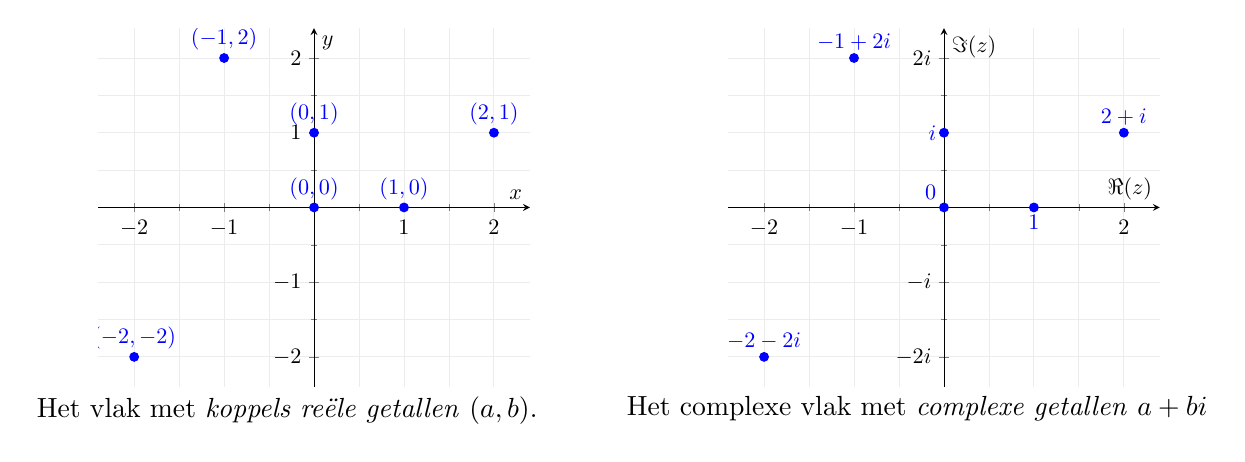
\begin{tikzpicture}[scale=0.8]
		\begin{scope}
			\begin{axis}[
				axis lines = center,
				grid=both,
				grid style={gray!15},
				minor tick num=1,
				% ticks=both,
				xlabel=$x$,
				ylabel=$y$,
				ytick ={-7,...,8}, 
				xtick ={-7,...,8}, 
				ymin=-2,ymax=+2,
				xmin=-2,xmax=+2,
				enlargelimits=true, 
				]
				
				\addplot [blue, mark = *] coordinates {( 0, 0)} node[above] {$(0,0)$};
				\addplot [blue, mark = *] coordinates {( 1, 0)} node[above] {$(1,0)$};
				\addplot [blue, mark = *] coordinates {( 0, 1)} node[above] {$(0,1)$};
				% \addplot [blue, mark = *] coordinates {( 2, 0)} node[above] {$(2,0)$};
				\addplot [blue, mark = *] coordinates {( 2, 1)} node[above] {$(2,1)$};
				\addplot [blue, mark = *] coordinates {( 2,-3)} node[above] {$(2,-3)$};
				\addplot [blue, mark = *] coordinates {(-1, 2)} node[above] {$(-1,2)$};
				\addplot [blue, mark = *] coordinates {(-2,-2)} node[above] {$(-2,-2)$};

			\end{axis}
			\node[below] at (3,0) {Het vlak met \textit{koppels reële getallen} $(a,b)$.};
		\end{scope}

		\begin{scope}[xshift=10cm]
			\begin{axis}[
				axis lines = center,
				grid=both,
				grid style={gray!15},
				minor tick num=1,
				% ticks=both,
				xlabel=$\Re(z)$,
				ylabel=$\Im(z)$,
				ytick ={-7,...,8}, yticklabels={$-7i$, $-6i$, $-5i$, $-4i$, $-3i$, $-2i$, $-i$, $0$, , $2i$, $3i$, $+3i$, $+4i$, $+5i$, $+6i$, $+7i$, $+8i$},
				xtick ={-3,...,3}, xticklabels={$-3$,$-2$,$-1$, , ,$2$,$3$},
				ymin=-2,ymax=+2,
				xmin=-2,xmax=+2,
				enlargelimits=true,
				]
				
				\addplot [blue, mark = *] coordinates {( 0, 0)} node[above left] {$0$};
				\addplot [blue, mark = *] coordinates {( 1, 0)} node[below] {$1$};
				\addplot [blue, mark = *] coordinates {( 0, 1)} node[left] {$i$};
				%\addplot [blue, mark = *] coordinates {( 2, 0)} node[above left] {$2$};
				\addplot [blue, mark = *] coordinates {( 2, 1)} node[above] {$2+i$};
				\addplot [blue, mark = *] coordinates {( 2,-3)} node[above] {$2-3i$};
				\addplot [blue, mark = *] coordinates {(-1, 2)} node[above] {$-1+2i$};
				\addplot [blue, mark = *] coordinates {(-2,-2)} node[above] {$-2-2i$};
			\end{axis}
			\node[below] at (3,0) {Het complexe vlak met \textit{complexe getallen} \(a+bi\)};
		\end{scope}
	\end{tikzpicture}
\end{image}


\end{hint}

\begin{oplossing}

Het complexe getal \(z = 1 + 2i\) heeft als reëel deel \( \Re(z) = \Re(1+2i) = 1\)  en als imaginair deel \( \Im(z)} = \Im(1+2i) = 2 \). 

We nemen 1 eenheid op de reële-as en 2 eenheden op de imaginaire as: 

\begin{image}
	\begin{tikzpicture}[>=stealth, scale=1.0]

		% Draw axes
		\draw[->] (-0.5,0) -- (3.0,0) node[right] {\(\mathrm{Re}(z)\)};
		\draw[->] (0,-0.5) -- (0,3.0) node[above] {\(\mathrm{Im}(z)\)};
		
		% Mark the point z = 1 + 2i
		\filldraw (1,2) circle (2pt) node[right] {\(z = 1 + 2i\)};
		
		% Dashed lines to show real and imaginary parts
		\draw[dashed] (1,2) -- (1,0) node[midway,right] {2};
		\draw[dashed] (1,0) -- (0,0) node[midway,below] {1};
		
		% Optionally, draw an arrow from origin to the point
		\draw[->] (0,0) -- (1,2);
		% You could label the magnitude if you like:
		% \node at (0.5,1.0) {\(\sqrt{1^2 + 2^2} = \sqrt{5}\)};
	
	\end{tikzpicture}
\end{image}

\end{oplossing}

\end{exercise}
\end{document}




\begin{exercise} Stel de volgende getallen voor in het complexe vlak. 
    \begin{itemize}
    \begin{question} \( 3+2i \)
    \begin{question} \( -3+2i\)
    \begin{question} \( 3 + 4i  \)
    \begin{question} \( 5 - 2i  \)
    \begin{question} \( -1-i \)
    \end{itemize}
    
\end{exercise}



\begin{exercise} Stel de volgende getallen voor in het complexe vlak. 
        
\begin{question} \( -2 + i  \)
\begin{question} \( 0    \)
\begin{question} \( -1 - 3i \)
\begin{question} \( -7i  \)
\begin{question} \( 7 + 2i  \)
    
\end{exercise}





\end{document}